\begin{figure}[h!]
\centering
% This file was created by matplotlib2tikz v0.6.17.
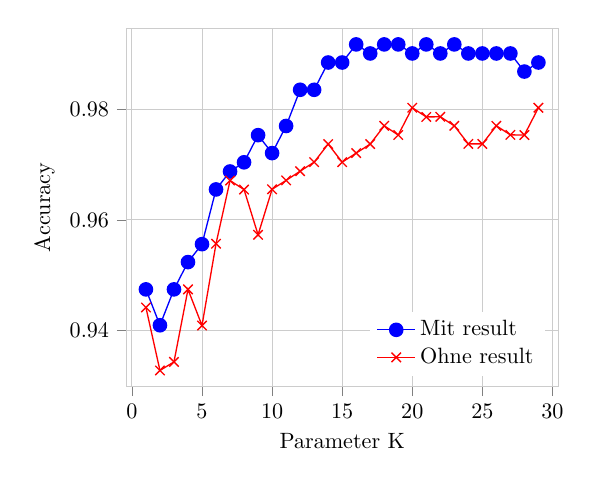
\begin{tikzpicture}[scale=.8,transform shape]

\begin{axis}[
xlabel={Parameter K},
ylabel={Accuracy},
xmin=-0.4, xmax=30.4,
ymin=0.92975, ymax=0.994758196721311,
tick align=outside,
tick pos=left,
xmajorgrids,
x grid style={white!80.0!black},
ymajorgrids,
y grid style={white!80.0!black},
axis line style={white!80.0!black},
legend entries={{Mit result},{Ohne result}},
legend cell align={left},
legend style={at={(0.97,0.03)}, anchor=south east, draw=none}
]
\addplot [semithick, blue, mark=*, mark size=3, mark options={solid}]
table {%
1 0.947404371584699
2 0.940901639344262
3 0.947404371584699
4 0.952349726775956
5 0.955601092896175
6 0.96551912568306
7 0.968770491803279
8 0.970437158469945
9 0.975355191256831
10 0.972103825136612
11 0.977021857923497
12 0.983579234972678
13 0.983579234972678
14 0.988524590163934
15 0.988524590163934
16 0.991803278688524
17 0.990163934426229
18 0.991803278688524
19 0.991803278688524
20 0.990163934426229
21 0.991803278688524
22 0.990163934426229
23 0.991803278688524
24 0.990163934426229
25 0.990163934426229
26 0.990163934426229
27 0.990163934426229
28 0.986885245901639
29 0.988524590163934
};
\addplot [semithick, red, mark=x, mark size=3, mark options={solid}]
table {%
1 0.944125683060109
2 0.932704918032787
3 0.934262295081967
4 0.947404371584699
5 0.940846994535519
6 0.95568306010929
7 0.967131147540984
8 0.965491803278688
9 0.957295081967213
10 0.965546448087432
11 0.967158469945355
12 0.968825136612022
13 0.970464480874317
14 0.973743169398907
15 0.970464480874317
16 0.972103825136612
17 0.973743169398907
18 0.977049180327869
19 0.975382513661202
20 0.980327868852459
21 0.978661202185792
22 0.978688524590164
23 0.977049180327869
24 0.973770491803279
25 0.973770491803279
26 0.977049180327869
27 0.975409836065574
28 0.975382513661202
29 0.980327868852459
};
\end{axis}

\end{tikzpicture}
\caption{\em Errechnete Fehlerraten unter der Variation der Anzahl der Nachbarn}
\label{fig:k_neighbours}
\end{figure}

\subsection{K-Nearest-Neighbour} \label{sec:kneighbour}
Neben der Support-Vector-Machine dient der Algorithmus K-Nearest-Neighbour ebenso gut zur Unterscheidung der zwei Klassen einer positiven und negativen Autismus-Diagnose. Im Rahmen der Auswertung des Algorithmus werden hierzu die Anzahl der $k$ nächsten Nachbarn variiert und eine Kreuzvalidierung der Daten durchgeführt.

Das Ergebnis des Algorithmus zeigt dabei nach Abbildung \ref{fig:k_neighbours}, dass bei einer Anzahl von $k=15$ Nachbarn für den Datensatz mit dem Merkmal \textit{result} eine Trennschärfe von bis zu 99\% erreicht werden kann. Im Vergleich dazu erreicht der Algorithmus ohne das Merkmal \textit{result} mit der Wahl $k=20$ eine Trennschärfe von 96\%. Die bessere Trennschärfe bei der Verwendung des zusätzlichen Merkmals ist dabei auf das Ergebnis aus der Datenanalyse zur Einteilung der Klassifikation anhand der Spalte \textit{result} zurückzuführen.
